% Options for packages loaded elsewhere
% Options for packages loaded elsewhere
\PassOptionsToPackage{unicode}{hyperref}
\PassOptionsToPackage{hyphens}{url}
%
\documentclass[
  10pt,
  ignorenonframetext,
  aspectratio=169,
  brazilian,
]{beamer}
\newif\ifbibliography
\usepackage{pgfpages}
\setbeamertemplate{caption}[numbered]
\setbeamertemplate{caption label separator}{: }
\setbeamercolor{caption name}{fg=normal text.fg}
\beamertemplatenavigationsymbolsempty
% remove section numbering
\setbeamertemplate{part page}{
  \centering
  \begin{beamercolorbox}[sep=16pt,center]{part title}
    \usebeamerfont{part title}\insertpart\par
  \end{beamercolorbox}
}
\setbeamertemplate{section page}{
  \centering
  \begin{beamercolorbox}[sep=12pt,center]{section title}
    \usebeamerfont{section title}\insertsection\par
  \end{beamercolorbox}
}
\setbeamertemplate{subsection page}{
  \centering
  \begin{beamercolorbox}[sep=8pt,center]{subsection title}
    \usebeamerfont{subsection title}\insertsubsection\par
  \end{beamercolorbox}
}
% Prevent slide breaks in the middle of a paragraph
\widowpenalties 1 10000
\raggedbottom
\AtBeginPart{
  \frame{\partpage}
}
\AtBeginSection{
  \ifbibliography
  \else
    \frame{\sectionpage}
  \fi
}
\AtBeginSubsection{
  \frame{\subsectionpage}
}
\usepackage{iftex}
\ifPDFTeX
  \usepackage[T1]{fontenc}
  \usepackage[utf8]{inputenc}
  \usepackage{textcomp} % provide euro and other symbols
\else % if luatex or xetex
  \usepackage{unicode-math} % this also loads fontspec
  \defaultfontfeatures{Scale=MatchLowercase}
  \defaultfontfeatures[\rmfamily]{Ligatures=TeX,Scale=1}
\fi
\usepackage{lmodern}

\usetheme[]{Madrid}
\ifPDFTeX\else
  % xetex/luatex font selection
\fi
% Use upquote if available, for straight quotes in verbatim environments
\IfFileExists{upquote.sty}{\usepackage{upquote}}{}
\IfFileExists{microtype.sty}{% use microtype if available
  \usepackage[]{microtype}
  \UseMicrotypeSet[protrusion]{basicmath} % disable protrusion for tt fonts
}{}
\makeatletter
\@ifundefined{KOMAClassName}{% if non-KOMA class
  \IfFileExists{parskip.sty}{%
    \usepackage{parskip}
  }{% else
    \setlength{\parindent}{0pt}
    \setlength{\parskip}{6pt plus 2pt minus 1pt}}
}{% if KOMA class
  \KOMAoptions{parskip=half}}
\makeatother


\usepackage{longtable,booktabs,array}
\newcounter{none} % for unnumbered tables
\usepackage{calc} % for calculating minipage widths
\usepackage{caption}
% Make caption package work with longtable
\makeatletter
\def\fnum@table{\tablename~\thetable}
\makeatother
\usepackage{graphicx}
\makeatletter
\newsavebox\pandoc@box
\newcommand*\pandocbounded[1]{% scales image to fit in text height/width
  \sbox\pandoc@box{#1}%
  \Gscale@div\@tempa{\textheight}{\dimexpr\ht\pandoc@box+\dp\pandoc@box\relax}%
  \Gscale@div\@tempb{\linewidth}{\wd\pandoc@box}%
  \ifdim\@tempb\p@<\@tempa\p@\let\@tempa\@tempb\fi% select the smaller of both
  \ifdim\@tempa\p@<\p@\scalebox{\@tempa}{\usebox\pandoc@box}%
  \else\usebox{\pandoc@box}%
  \fi%
}
% Set default figure placement to htbp
\def\fps@figure{htbp}
\makeatother



\ifLuaTeX
\usepackage[bidi=basic,shorthands=off]{babel}
\else
\usepackage[bidi=default,shorthands=off]{babel}
\fi
\ifLuaTeX
  \usepackage{selnolig} % disable illegal ligatures
\fi


\setlength{\emergencystretch}{3em} % prevent overfull lines

\providecommand{\tightlist}{%
  \setlength{\itemsep}{0pt}\setlength{\parskip}{0pt}}



 


% ---- CORES ----
\definecolor{CustomGreen}{HTML}{1B5E20}
\definecolor{CustomGreenLight}{HTML}{388E3C}
\definecolor{CustomGreenDark}{HTML}{0D3B12}
% ---- TEMA BEAMER ----
\setbeamercolor{structure}{fg=CustomGreen}
\setbeamercolor{title}{fg=white,bg=CustomGreen}
\setbeamercolor{frametitle}{fg=white,bg=CustomGreen}
\setbeamercolor{block title}{fg=white,bg=CustomGreen}
\setbeamercolor{block body}{fg=black,bg=white}
\setbeamertemplate{navigation symbols}{}
\setbeamertemplate{itemize item}{\color{CustomGreen}\small$\bullet$}
\setbeamertemplate{itemize subitem}{\color{CustomGreen}–}
\setbeamertemplate{itemize subsubitem}{\color{CustomGreen}}
\setbeamertemplate{footline}[frame number]
% ---- LOGO ----
\usepackage{graphicx}
\logo{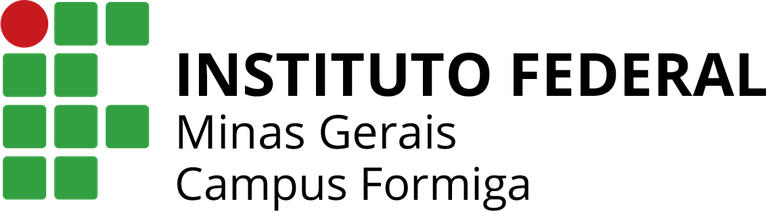
\includegraphics[height=1cm]{IFMG.png}}
\makeatletter
\@ifpackageloaded{caption}{}{\usepackage{caption}}
\AtBeginDocument{%
\ifdefined\contentsname
  \renewcommand*\contentsname{Índice}
\else
  \newcommand\contentsname{Índice}
\fi
\ifdefined\listfigurename
  \renewcommand*\listfigurename{Lista de Figuras}
\else
  \newcommand\listfigurename{Lista de Figuras}
\fi
\ifdefined\listtablename
  \renewcommand*\listtablename{Lista de Tabelas}
\else
  \newcommand\listtablename{Lista de Tabelas}
\fi
\ifdefined\figurename
  \renewcommand*\figurename{Figura}
\else
  \newcommand\figurename{Figura}
\fi
\ifdefined\tablename
  \renewcommand*\tablename{Tabela}
\else
  \newcommand\tablename{Tabela}
\fi
}
\@ifpackageloaded{float}{}{\usepackage{float}}
\floatstyle{ruled}
\@ifundefined{c@chapter}{\newfloat{codelisting}{h}{lop}}{\newfloat{codelisting}{h}{lop}[chapter]}
\floatname{codelisting}{Listagem}
\newcommand*\listoflistings{\listof{codelisting}{Lista de Listagens}}
\makeatother
\makeatletter
\makeatother
\makeatletter
\@ifpackageloaded{caption}{}{\usepackage{caption}}
\@ifpackageloaded{subcaption}{}{\usepackage{subcaption}}
\makeatother

\usepackage{bookmark}
\IfFileExists{xurl.sty}{\usepackage{xurl}}{} % add URL line breaks if available
\urlstyle{same}
\hypersetup{
  pdftitle={Corrupção e composição dos gastos governamentais: evidências a partir do Programa de Fiscalização por Sorteios Públicos da Controladoria-Geral da União},
  pdfauthor={Olavo Venturim Caldas \textbar{} Cristiano Machado Costa \textbar{} Marcelo Sanches Pagliarussi},
  pdflang={pt-BR},
  hidelinks,
  pdfcreator={LaTeX via pandoc}}


\title{\texorpdfstring{Corrupção e composição dos gastos governamentais:
evidências a partir do Programa de Fiscalização por Sorteios Públicos da
Controladoria-Geral da
União}{Corrupção e composição dos gastos governamentais: evidências a partir do Programa de Fiscalização por Sorteios Públicos da Controladoria-Geral da União}}
\author{Olavo Venturim Caldas \textbar{} Cristiano Machado Costa
\textbar{} Marcelo Sanches Pagliarussi}
\date{}
\institute{Disciplina: Econometria aplicada a Finanças \textbar{}
Prof.~Dr.~Washington Santos da Silva}

\begin{document}
\frame{\titlepage}


\begin{frame}
Rev.~Adm. Pública 50 (2) - Mar-Apr 2016
\end{frame}

\begin{frame}{Introdução}
\protect\phantomsection\label{introduuxe7uxe3o}
\begin{itemize}
\item
  A corrupção representa um problema relevante para a gestão dos
  recursos públicos e pode afetar a eficiência da atuação governamental.
\item
  A literatura econômica relaciona a corrupção a diferentes resultados,
  como menor crescimento econômico, redução dos investimentos e
  alterações na arrecadação e na aplicação dos recursos públicos.
\item
  No caso dos municípios brasileiros, a alocação dos recursos ocorre
  dentro de um ambiente institucional específico, marcado por regras
  constitucionais e legais que estabelecem limites e vinculações para
  determinadas despesas.
\item
  Essas restrições são particularmente importantes nas áreas de saúde e
  educação.
\item
  Apesar dessas restrições, os gestores municipais possuem diferentes
  possibilidades de alocação dos recursos entre funções e categorias de
  despesas.
\item
  Diante disso, torna-se relevante investigar se a corrupção está
  associada à forma como os municípios brasileiros distribuem seus
  gastos públicos.
\end{itemize}
\end{frame}

\begin{frame}{Objetivo e questão de pesquisa}
\protect\phantomsection\label{objetivo-e-questuxe3o-de-pesquisa}
\textbf{Objetivo:}

\begin{itemize}
\tightlist
\item
  Investigar a relação entre corrupção e composição dos gastos públicos
  dos municípios brasileiros.
\end{itemize}

\textbf{Questão de pesquisa:}

\begin{itemize}
\tightlist
\item
  A corrupção está relacionada à forma como os municípios brasileiros
  alocam seus gastos públicos?
\end{itemize}

Para responder à questão, os autores utilizam informações sobre
irregularidades identificadas pela CGU e dados sobre as despesas
municipais, analisando a relação entre corrupção e diferentes categorias
de gastos públicos.
\end{frame}

\begin{frame}{Características relevantes do ambiente institucional
brasileiro}
\protect\phantomsection\label{caracteruxedsticas-relevantes-do-ambiente-institucional-brasileiro}
\textbf{Despesas municipais e transferências da União}

\begin{itemize}
\item
  A legislação brasileira organiza as despesas municipais por diferentes
  funções de governo.
\item
  Saúde e educação possuem participação elevada na composição das
  despesas municipais.
\item
  Em 2010, essas duas funções representavam aproximadamente 48\% das
  despesas municipais.
\item
  As transferências da União possuem participação significativa no
  financiamento dessas áreas, evidenciando a dependência dos municípios
  em relação às transferências intergovernamentais.
\end{itemize}

\textbf{Limites obrigatórios de gastos públicos municipais}

\begin{itemize}
\item
  Os municípios estão sujeitos a regras que limitam sua
  discricionariedade na alocação dos recursos.
\item
  Educação: aplicação mínima de 25\% das receitas de impostos e
  transferências.
\item
  Saúde: aplicação mínima de 15\% das receitas de impostos e
  transferências.
\item
  A Lei de Responsabilidade Fiscal estabelece limite de 60\% da receita
  para despesas com pessoal.
\item
  Apesar das vinculações, permanece espaço para decisões sobre como os
  recursos serão utilizados dentro de cada função.
\end{itemize}
\end{frame}

\begin{frame}{Características relevantes do ambiente institucional
brasileiro}
\protect\phantomsection\label{caracteruxedsticas-relevantes-do-ambiente-institucional-brasileiro-1}
\textbf{Programa de Fiscalização por Sorteios Públicos da CGU}

\begin{itemize}
\item
  Criado em 2003, o programa tem como objetivo fiscalizar a aplicação de
  recursos públicos federais e combater irregularidades na administração
  pública.
\item
  Os municípios são selecionados por meio de sorteios públicos, buscando
  reduzir a possibilidade de seleção direcionada das unidades
  fiscalizadas.
\item
  As equipes da CGU realizam auditorias e analisam documentos,
  processos, recursos financeiros, obras e serviços públicos.
\item
  As fiscalizações produzem relatórios com as irregularidades
  identificadas e respectivas evidências.
\item
  Os dados da CGU permitem construir uma medida de corrupção baseada em
  irregularidades efetivamente constatadas, em vez de índices de
  percepção.
\end{itemize}
\end{frame}

\begin{frame}{Estudos anteriores}
\protect\phantomsection\label{estudos-anteriores}
\begin{itemize}
\item
  Mauro (1998): corrupção → menor gasto em Educação e Saúde.
\item
  Gupta et al.~(2001): corrupção → maior gasto militar.
\item
  Estudos brasileiros relacionam corrupção a:

  \begin{itemize}
  \tightlist
  \item
    incentivos e discricionariedade dos gestores;
  \item
    transferências públicas;
  \item
    piora dos resultados educacionais;
  \item
    redução da atividade empresarial.
  \end{itemize}
\item
  Lacuna: ausência de análise sobre corrupção e composição das despesas
  municipais.
\end{itemize}
\end{frame}

\begin{frame}{Referencial teórico e desenvolvimento de hipóteses}
\protect\phantomsection\label{referencial-teuxf3rico-e-desenvolvimento-de-hipuxf3teses}
\textbf{Quadro teórico}

\begin{itemize}
\tightlist
\item
  A corrupção é favorecida pela combinação de poder discricionário,
  oportunidade de extração de renda e instituições frágeis.
\item
  Pela teoria de Rent-Seeking, agentes privados competem por benefícios
  e tratamento preferencial na utilização dos recursos públicos.
\item
  O modelo considera que políticos e burocratas podem ser agentes da
  corrupção.
\end{itemize}

\textbf{Argumento central}

\begin{itemize}
\tightlist
\item
  A obrigatoriedade de gastos pode tornar Saúde e Educação setores mais
  atrativos para práticas de Rent-Seeking.
\end{itemize}
\end{frame}

\begin{frame}{Desenvolvimento das hipóteses}
\protect\phantomsection\label{desenvolvimento-das-hipuxf3teses}
\textbf{Educação e Saúde}

\begin{itemize}
\tightlist
\item
  H1: corrupção em educação → aumento das despesas municipais em
  educação.
\item
  H2: corrupção em saúde → aumento das despesas municipais em saúde.
\item
  H3: corrupção em educação → aumento das despesas de educação
  financiadas por transferências da União.
\item
  H4: corrupção em saúde → aumento das despesas de saúde financiadas por
  transferências da União.
\end{itemize}

\textbf{Assistência Social}

\begin{itemize}
\tightlist
\item
  H5: corrupção em assistência social → redução das despesas municipais
  em assistência social.
\item
  H6: corrupção em assistência social → redução das despesas de
  assistência social financiadas por transferências da União.
\end{itemize}

\textbf{Relação esperada}

\begin{itemize}
\tightlist
\item
  H1--H4: relação esperada positiva para Educação e Saúde.
\item
  H5--H6: relação esperada negativa para Assistência Social.
\end{itemize}
\end{frame}

\begin{frame}{Dados: fontes e construção}
\protect\phantomsection\label{dados-fontes-e-construuxe7uxe3o}
\textbf{A base foi construída a partir de quatro fontes principais:}

\begin{itemize}
\tightlist
\item
  CGU: auditorias do Programa de Fiscalização por Sorteios Públicos
  (PFSP).
\item
  Portal da Transparência: transferências da União aos municípios.
\item
  STN/Finbra: despesas orçamentárias municipais por função de governo.
\item
  IBGE/IPEA: indicadores socioeconômicos e demográficos.
\end{itemize}

\textbf{Medida de corrupção}

\begin{itemize}
\tightlist
\item
  Aplicação de Text Mining às constatações da CGU.
\item
  Tokenização e stemming para identificar termos associados a fraudes.
\item
  Exemplos: notas frias, empresas fantasmas, superfaturamento e
  licitações simuladas.
\end{itemize}
\end{frame}

\begin{frame}{Unidade de observação}
\protect\phantomsection\label{unidade-de-observauxe7uxe3o}
\begin{itemize}
\tightlist
\item
  Unidade de análise: município brasileiro em determinado ano \((i,t)\).
\item
  O ano \(t\) corresponde ao período em que o município foi sorteado e
  fiscalizado pela CGU.
\end{itemize}

\textbf{Defasagem temporal}

\begin{itemize}
\tightlist
\item
  As irregularidades identificadas refletem práticas ocorridas antes da
  auditoria.
\item
  Por isso, despesas, transferências e PIB consideram:

  \begin{itemize}
  \tightlist
  \item
    ano da fiscalização \((t)\);
  \item
    ano anterior \((t-1)\).
  \end{itemize}
\end{itemize}

A estrutura busca compatibilizar o período das irregularidades com os
dados fiscais e econômicos.
\end{frame}

\begin{frame}{Período e amostra}
\protect\phantomsection\label{peruxedodo-e-amostra}
\textbf{Período}

\begin{itemize}
\tightlist
\item
  20º ao 33º sorteio do PFSP.
\item
  2006--2010, com dados fiscais de 2005--2010.
\end{itemize}

\textbf{Amostra}

\begin{itemize}
\tightlist
\item
  840 municípios.
\item
  Municípios com até 500 mil habitantes.
\item
  Capitais estaduais excluídas.
\item
  39 municípios foram sorteados mais de uma vez.
\end{itemize}

\textbf{Tratamento dos dados}

\begin{itemize}
\tightlist
\item
  Exclusão do Bolsa Família.
\item
  Exclusão de falhas formais ou informativas.
\item
  Exclusão de registros com inconsistências ou omissões contábeis.
\end{itemize}
\end{frame}

\begin{frame}{Variáveis dependentes}
\protect\phantomsection\label{variuxe1veis-dependentes}
Foram estimados dois grupos de modelos:

\textbf{Modelo 1 --- Despesas municipais}

\[
Y_{it}=\frac{\text{Despesa municipal}_{it}}{\text{PIB}_{it}}
\]

\begin{itemize}
\tightlist
\item
  Despesa total ou por função:

  \begin{itemize}
  \tightlist
  \item
    Educação;
  \item
    Saúde;
  \item
    Assistência Social
  \end{itemize}
\end{itemize}

\textbf{Modelo 2 --- Transferências da União}

\[
Y_{it}=\frac{\text{Transferências federais}_{it}}{\text{PIB}_{it}}
\]

\begin{itemize}
\tightlist
\item
  Valores em termos reais, deflacionados pelo IPCA.
\end{itemize}
\end{frame}

\begin{frame}{Variáveis explicativas e controles}
\protect\phantomsection\label{variuxe1veis-explicativas-e-controles}
\textbf{Variável de interesse}

\[
corrup_{it}=
\frac{\text{Constatações classificadas como corrupção}}
{\text{Total de constatações}}
\]

\begin{itemize}
\tightlist
\item
  Medida por município e função de governo.
\end{itemize}

\textbf{Variáveis de controle}

\begin{itemize}
\tightlist
\item
  Gini: desigualdade de renda.
\item
  PIB per capita: nível de desenvolvimento econômico.
\item
  População: tamanho do município.
\item
  Urbanização: proporção da população urbana.
\item
  Transferências/Despesa: participação dos repasses federais no
  orçamento.
\end{itemize}
\end{frame}

\begin{frame}{Modelo econométrico}
\protect\phantomsection\label{modelo-economuxe9trico}
\textbf{Método}

\begin{itemize}
\tightlist
\item
  Mínimos Quadrados Ordinários (MQO).

  \begin{itemize}
  \tightlist
  \item
    ``Nesse caso, o método de mínimos quadrados ordinários é adequado,
    na medida em que os municípios são sorteados aleatoriamente e com
    reposição ao longo dos anos, conferindo independência entre as
    observações e eliminando correlações entre erros ao longo dos anos''
    (Wooldridge, 2010)
  \end{itemize}
\item
  Erros-padrão robustos à heterocedasticidade e autocorrelação.
\item
  Estrutura de Pooled Cross-Sections.
\end{itemize}

\textbf{Despesas municipais}

\[
Desppib_{it}=
\beta_0+\beta_1corrup_{it}
+\beta_2Gini_{it}
+\beta_3PIB_{it}
+\beta_4pop_{it}
+\beta_5urban_{it}
+\beta_6transf\_despesa_{it}
+\varepsilon_{it}
\]

\textbf{Transferências da União}

\[
Transfpib_{it}=
\beta_0+\beta_1corrup_{it}
+\beta_2Gini_{it}
+\beta_3PIB_{it}
+\beta_4pop_{it}
+\beta_5urban_{it}
+\varepsilon_{it}
\]

O coeficiente central é \(\beta_1\): relação entre corrupção e alocação
dos recursos públicos.
\end{frame}

\begin{frame}{Diagnóstico descritivo}
\protect\phantomsection\label{diagnuxf3stico-descritivo}
\begin{itemize}
\tightlist
\item
  Transferências da União representam, em média, 60\% das despesas
  municipais.
\item
  15,65\% das Ordens de Serviço apresentam constatações classificadas
  como corrupção.
\item
  Maior incidência:

  \begin{itemize}
  \tightlist
  \item
    Saúde: 18,94\%;
  \item
    Educação: 17,54\%.
  \end{itemize}
\item
  Menor incidência:

  \begin{itemize}
  \tightlist
  \item
    Assistência Social: 1,25\%.
  \end{itemize}
\end{itemize}

A corrupção concentra-se principalmente em Saúde e Educação.
\end{frame}

\begin{frame}{Corrupção e despesas municipais}
\protect\phantomsection\label{corrupuxe7uxe3o-e-despesas-municipais}
\begin{columns}[T]
\begin{column}{0.5\linewidth}
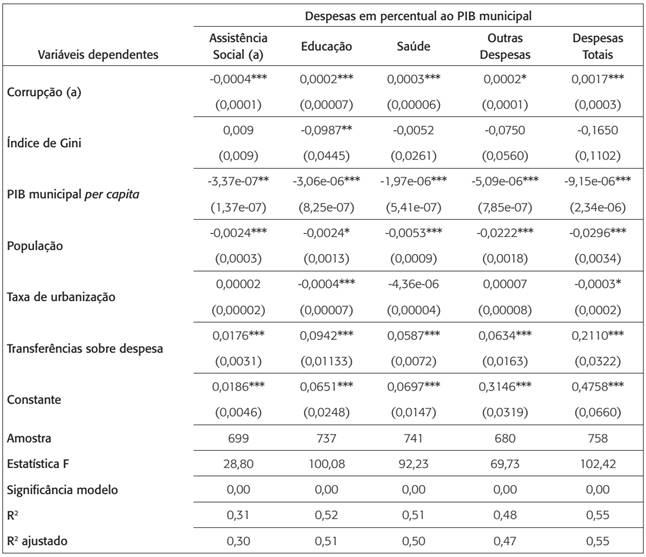
\includegraphics[width=1\linewidth,height=\textheight,keepaspectratio]{Modelo_despesas.jpg}

\centering{Fonte: Elaborado pelos autores}
\end{column}

\begin{column}{0.5\linewidth}
\begin{itemize}
\tightlist
\item
  Despesa Total/PIB: \(\beta=0,0017\) (\(p<0,01\)).
\item
  Educação/PIB: \(\beta=0,0002\) (\(p<0,01\)).
\item
  Saúde/PIB: \(\beta=0,0003\) (\(p<0,01\)).
\item
  Assistência Social: associação negativa.
\end{itemize}

Resultados:

\begin{itemize}
\tightlist
\item
  H1 e H2 confirmadas.
\item
  H5 confirmada.
\item
  Maior corrupção está associada à expansão das despesas totais,
  Educação e Saúde.
\end{itemize}

No Brasil, a corrupção parece expandir o orçamento, em vez de apenas
redistribuí-lo entre funções.
\end{column}
\end{columns}
\end{frame}

\begin{frame}{Corrupção e transferências da União}
\protect\phantomsection\label{corrupuxe7uxe3o-e-transferuxeancias-da-uniuxe3o}
\begin{columns}[T]
\begin{column}{0.5\linewidth}
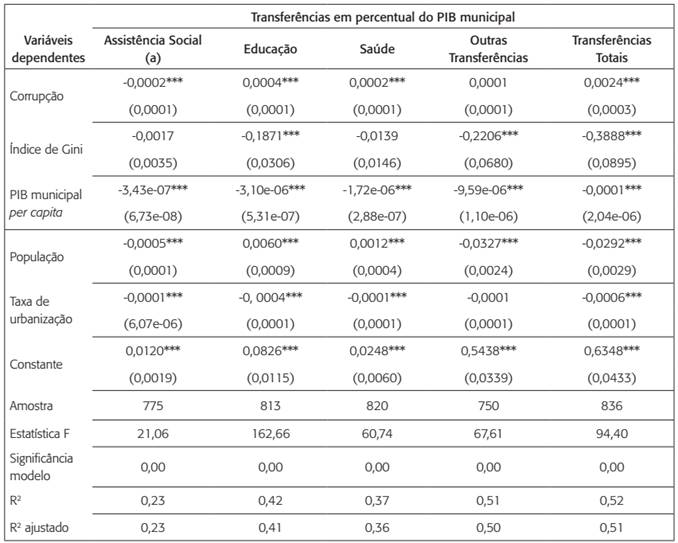
\includegraphics[width=1\linewidth,height=\textheight,keepaspectratio]{Modelo_Transf..jpg}

\centering{Fonte: Elaborado pelos autores}
\end{column}

\begin{column}{0.5\linewidth}
\begin{itemize}
\tightlist
\item
  Transferências Totais/PIB: \(\beta=0,0024\) (\(p<0,01\)).
\item
  Educação/PIB: \(\beta=0,0004\) (\(p<0,01\)).
\item
  Saúde/PIB: \(\beta=0,0002\) (\(p<0,01\)).
\item
  Assistência Social/PIB: \(\beta=-0,0002\) (\(p<0,01\)).
\end{itemize}

Resultados:

\begin{itemize}
\tightlist
\item
  H3 e H4 confirmadas.
\item
  H6 confirmada.
\item
  Corrupção associa-se a maiores transferências para Saúde e Educação.
\end{itemize}

Os repasses federais ampliam os recursos disponíveis nessas funções.
\end{column}
\end{columns}
\end{frame}

\begin{frame}{Testes de robustez e mecanismo}
\protect\phantomsection\label{testes-de-robustez-e-mecanismo}
\textbf{Testes de robustez}

\begin{itemize}
\tightlist
\item
  Exclusão dos 39 municípios sorteados mais de uma vez:

  \begin{itemize}
  \tightlist
  \item
    resultados permanecem significativos.
  \end{itemize}
\item
  Normalização pela despesa total:

  \begin{itemize}
  \tightlist
  \item
    Educação e Assistência mantêm os resultados;
  \item
    Saúde perde significância.
  \end{itemize}
\end{itemize}

\textbf{Mecanismo}

\begin{itemize}
\tightlist
\item
  A corrupção não parece simplesmente deslocar recursos entre funções.
\item
  Municípios mais corruptos apresentam maior despesa total em relação ao
  PIB.
\item
  Parte dessa expansão é direcionada para Saúde e Educação.
\end{itemize}

Corrupção associada à expansão do orçamento, e não apenas à sua
redistribuição.
\end{frame}

\begin{frame}{Conclusão}
\protect\phantomsection\label{conclusuxe3o}
\begin{itemize}
\tightlist
\item
  Corrupção implica em maiores despesas e transferências em Saúde e
  Educação, divergindo da literatura internacional.
\item
  Regras fiscais brasileiras direcionam recursos para setores com maior
  volume de recursos vinculados.
\item
  A corrupção expande o orçamento municipal, sem evidência de melhoria
  proporcional dos serviços públicos.
\item
  Novas fontes de recursos, como emendas e royalties, podem ampliar a
  exposição a desvios.
\item
  Recomenda-se fortalecer:

  \begin{itemize}
  \tightlist
  \item
    transparência;
  \item
    integridade;
  \item
    controle interno;
  \item
    mecanismos de fiscalização.
  \end{itemize}
\end{itemize}

O ambiente institucional condiciona a relação entre corrupção e alocação
dos gastos públicos.
\end{frame}

\begin{frame}{Análise Crítica Econométrica}
\protect\phantomsection\label{anuxe1lise-cruxedtica-economuxe9trica}
\emph{O modelo utilizado é coerente com o problema investigado e com os
dados?}

\begin{itemize}
\tightlist
\item
  Sim. O uso de MQO é compatível com o desenho da pesquisa.
\item
  A normalização das despesas e transferências pelo PIB controla
  diferenças de escala entre municípios.
\end{itemize}

\emph{Os coeficientes e demais resultados são interpretados
adequadamente?}

\begin{itemize}
\tightlist
\item
  Sim. Os autores consideram sinal, significância estatística e contexto
  institucional.
\item
  O teste de robustez mostra que os resultados são sensíveis à forma de
  normalização.
\end{itemize}

\emph{Quais conclusões são efetivamente sustentadas pelos resultados?}

\begin{itemize}
\tightlist
\item
  Corrupção está associada a maiores despesas e transferências em Saúde
  e Educação.
\item
  Há associação negativa com Assistência Social.
\item
  Os resultados indicam associação, não necessariamente causalidade.
\end{itemize}
\end{frame}

\begin{frame}{Análise Crítica Econométrica}
\protect\phantomsection\label{anuxe1lise-cruxedtica-economuxe9trica-1}
\emph{Algum pressuposto, característica dos dados ou problema
econométrico merece atenção?}

\begin{itemize}
\tightlist
\item
  Possível endogeneidade por variáveis omitidas.
\item
  A medida de corrupção baseada em Text Mining pode apresentar erro de
  mensuração.
\item
  Os erros-padrão robustos são um ponto positivo.
\end{itemize}

\emph{Existem limitações importantes para a interpretação dos
resultados?}

\begin{itemize}
\tightlist
\item
  Validade externa restrita a municípios de até 500 mil habitantes.
\item
  A variável representa corrupção detectada, não a corrupção total
  existente.
\item
  Os resultados são sensíveis ao denominador utilizado nas variáveis
  dependentes.
\end{itemize}
\end{frame}




\end{document}
